\documentclass[11pt,a4paper,titlepage, ngerman]{article}

\usepackage[utf8]{inputenc}	% Diese Pakete sind
\usepackage[T1]{fontenc}		% für die Verwendung 
\usepackage{ngerman}			% von Umlauten im tex-file
\usepackage{lmodern}			% Schriftart, die am Bildschirm besser lesbar ist
\usepackage{graphicx}			% Zum Einbinden von Formeln
\usepackage{url}					% Zur Darstellung von Webadressen
\usepackage{siunitx}
\usepackage{amsmath}			% für equation*
\usepackage{subcaption}
\usepackage{wrapfig}

\newcommand{\refeq}[1]{Gl. (\ref{eq:#1})}
\newcommand{\reffig}[1]{Fig. \ref{fig:#1}}
\newcommand{\reftab}[1]{Tab. \ref{tab:#1}}

\begin{document}
	
	\tableofcontents
	\newpage
	
	\section{Fermi}
	\begin{figure}[ht]
		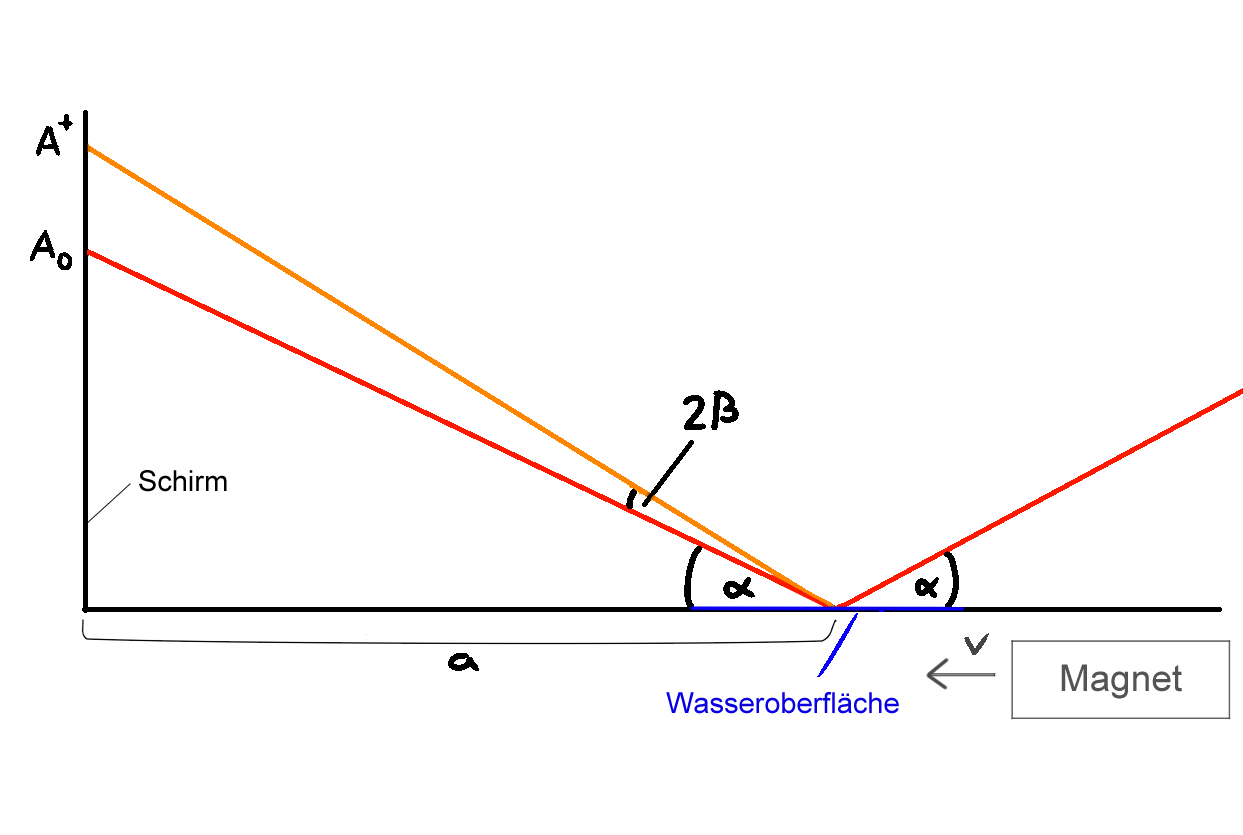
\includegraphics[width=\textwidth]{SkizzeFermi1.png}
		\caption{Skizze zum Versuch insgesammt}
		\label{fig:Fermi1}
	\end{figure}
	\begin{figure}[ht]
		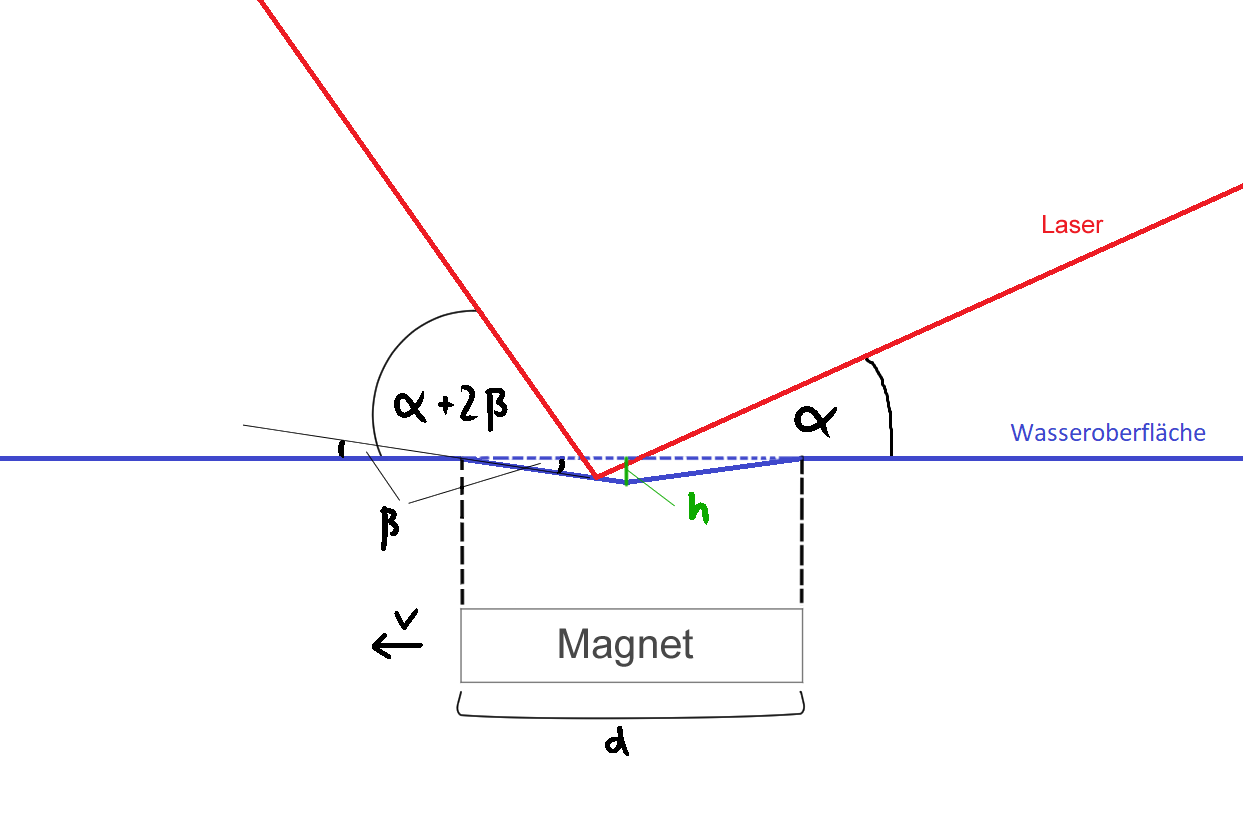
\includegraphics[width=\textwidth]{SkizzeFermi2.png}
		\caption{Skizze nahe beim Magneten}
		\label{fig:Fermi2}
	\end{figure}
	Es folgen die folgenden grundlegenden Gleichungen aus Fig. \ref{fig:Fermi1}
	\begin{align}
		\tan \alpha &= \frac{A_0}{a}
		\label{eq:schirm1}\\
		\tan (\alpha + 2 \beta) &= \frac{A^+}{a};\quad A^+ = A_0+\Delta A
		\label{eq:schirm2}
	\end{align}
	und aus Fig. \ref{fig:Fermi2}
	\begin{align}
		\tan \beta = \frac{2 h}{d}.
		\label{eq:kruemmung}
	\end{align}
	Wobei in \reffig{Fermi2} das Wasser in die andere Richtung gekrümmt ist.
	
	Stellt man \refeq{kruemmung} nach der gesuchten Größe $h$ um und setzt geeignet \refeq{schirm1} und \refeq{schirm2} ein, so folgt:
	\begin{align}
		\tan \beta = \frac{2h}{d} \Leftrightarrow h &= \frac{d}{2} \tan \beta\\
		&= \frac{d}{2} \tan \left( \frac{1}{2}\arctan \left( \frac{A^+}{a}\right) - \frac{\alpha}{2}\right)\\
		&= \frac{d}{2} \tan \left( \frac{\arctan \left( \frac{A^+}{a}\right) - \arctan\left( \frac{A_0}{a}\right)}{2} \right)
	\end{align}
	
	Mit den abgeschätzten Werten
	\begin{equation}
		a = \SI{3,5}{\meter};\quad
		A_0 = \SI{1,2}{\meter};\quad
		\Delta A = \SI{3}{\centi\meter};\quad
		d = \SI{1}{\centi\meter}
	\end{equation}
	ist $h \approx \SI{19}{\micro\meter}$.
	
	\begin{figure}[ht]
		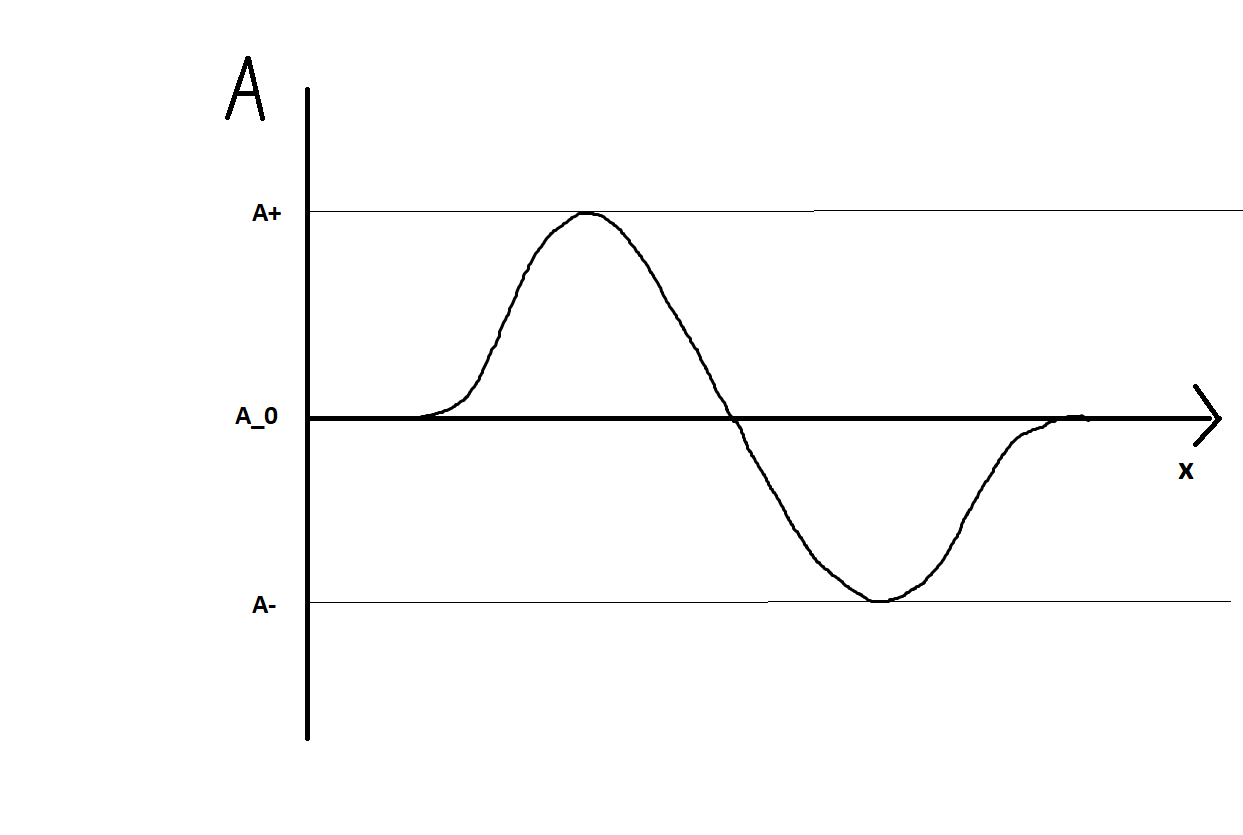
\includegraphics[width=\textwidth]{SkizzeZeitverlaufLichtpunktWasser.png}
		\caption{Verlauf der Position des Lichtpunktes auf dem Schirm gegen die Zeit.}
		\label{fig:zeitverlauf}
	\end{figure}
	
	Der Magnet wird wie in \reffig{Fermi2} mit einer konstanten Geschwindigkeit nach links gezogen.
	Da wie in \reffig{zeitverlauf} zu erkennen ist der Lichtpunkt erst nach oben ausschlägt, muss auch der Laserstrahl erst auf eine wie in \reffig{Fermi2} gezeigte Steigung treffen.
	Dabei wird in der Fermi-Abschätzung die Steigung als etwa konstant angesehen.
	Damit ist klar, dass sich eine leichte Vertiefung im Wasser durch den Magneten bilden muss.
	Daraus folgt wiederum, dass Wasser von einem Magnetfeld abgestoßen und so Diamagnetisch ist.
	
	Bei MaCl2$_2$ ist der Effekt umgekehrt und deutlich stärker.
	Dass bedeutet der Stoff bildet einen Hügel und ist damit Paramagnetisch.
	Die Höhe beläuft sich damit bei $\Delta A = \SI{0,7}{\meter}$ auf $h \approx \SI{420}{\micro\meter}$.
	Dadurch zeigt sich, dass paramagnetische Effekte deutlich stärker als diamagnetische sind.
	
	%%%%%%%%%%%%%%%%%%%%%%%%%%%%%%%%%%%%%%%%%%%%%%%%%%%%%%%%%%%%%%%%%%%%%%%%%%%%%%%%%%%%%%%%%%%%%%%%%%%%%%%%%%%%%%
	
	\section{Magnetwaage}
	\begin{figure}[ht]
		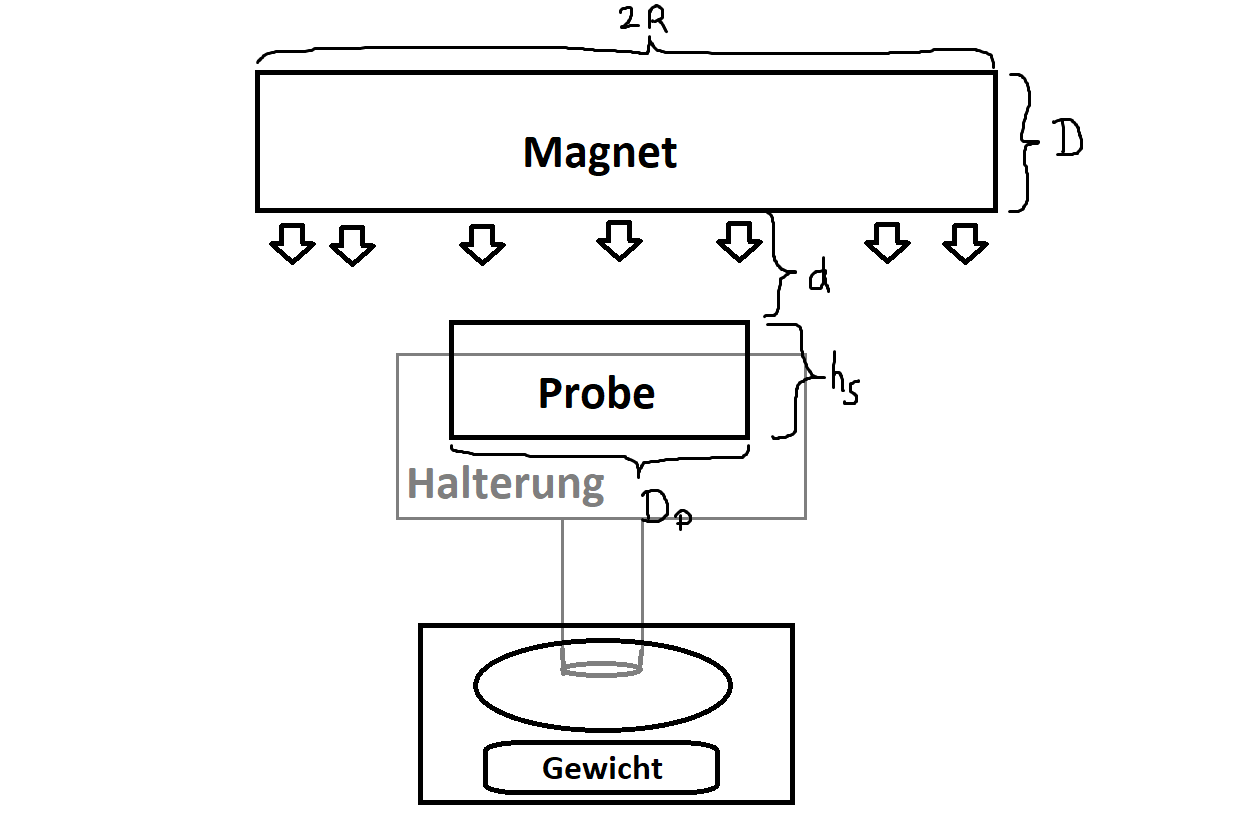
\includegraphics[width=\textwidth]{SkizzeMagnetwaage.png}
		\caption{Skizze zum Fallrohr.}
		\label{fig:magnetwaage}
	\end{figure}
	Wie in \reffig{magnetwaage} dargestellt, wird eine Probe in einem festen Abstand $d\approx\SI{1}{\milli\meter}$ unter einen starken Magneten plaziert und die Gewichtsänderung betrachtet.
	Da auch die Halterung magnetischen Effekten unterliegt, wird jeweils ein Referenzwert ohne Probe gemessen.
	Die Volumensuszeptibilität ist gegeben durch
	\begin{equation}
		\chi_V = \frac{2 \cdot \mu_0 \cdot \Delta m \cdot g}{V_S \cdot \frac{\partial\,B^2_z}{\partial\,z}},
	\end{equation}
	wobei näherungsweise gilt
	\begin{equation}
		\frac{\partial\,B^2_z}{\partial\,z} \approx \frac{B_z^2(d) - B_z^2(d+h_s)}{h_s}
	\end{equation}
	mit $h_s$ ist die Höhe der Probe und $d$ ist der Abstand der Probe zum Magneten.
	Gemessen 
	Für das Magnetfeld gilt
	\begin{equation}
		B(z) = \frac{B_r}{2}\left( \frac{D+z}{\sqrt{R^2 + (D+z)^2}} - \frac{z}{\sqrt{R^2 + z^2}}\right)
	\end{equation}
	mit speziefisch $B_r = \SI{1,87+-0,1}{T}$, sowie Radius $R = \SI{30}{\milli\meter}$ und Dicke $D = \SI{15}{\milli\meter}$.
	
	Rechnet man eine Formel nach der anderen aus, so bekommt man für jedes Material eine Volumensuszeptibilität.
	Insgesammt ergibt sich
	\begin{equation}
		\chi_V = \gamma \frac{\Delta m}{B_r^2}
	\end{equation}
	mit den Konstanten
	\begin{equation*}
		\gamma = \frac{8 \cdot \mu_0\cdot g \cdot h_S}{V_S \cdot \alpha};\quad
		\alpha = \left( B_z^{'}(d)\right)^2-\left( B_z^{'}(d+h_S)\right) ^2;\quad
		B_z^{'}(z) = \frac{D+z}{\sqrt{R^2 + (D+z)^2}} - \frac{z}{\sqrt{R^2+z^2}}
	\end{equation*}.
	
	Die Unsicherheit $u(\chi_V)$ berechnet sich folgendermaßen:
	\begin{equation}
		u(\chi_V) = \gamma\sqrt{\left( \frac{u(\Delta m)}{B_z^2}\right) ^2+\left( \frac{\Delta m}{2B_z^3}u(B_r)\right) ^2}
	\end{equation}
	
	Es folgen die Volumensuszeptibilitäten für die untersuchten Stoffe.
	%\begin{table}[S|S|S]
	%	Aluminium & Graphit & Glas \\
	%	\SI{13,79E-06 +- 4,61E-06}{} & \SI{value}{634,42E-06+-17,578E-06}{} & \SI{11,60E-06+-2,92E-06}{}
	%\end{table}
	
	\section{Schaukel}
	\begin{figure}[ht]
		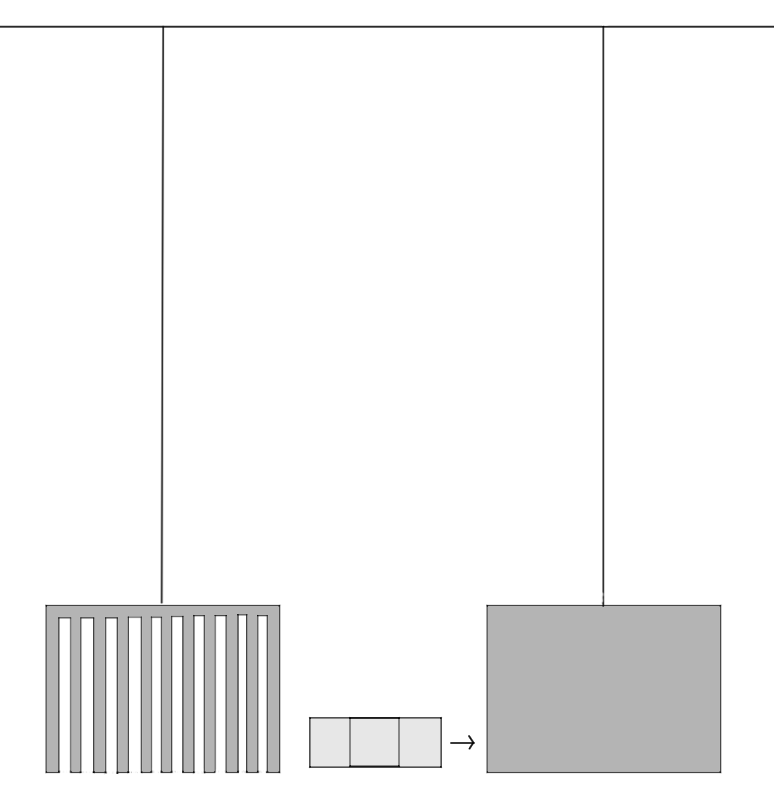
\includegraphics[width=\textwidth]{Alu-Platte.png}
		\caption{Skizze zum Fallrohr.}
		\label{fig:schaukel}
	\end{figure}
	
	\section{Fallrohr}
	\begin{figure}[ht]
		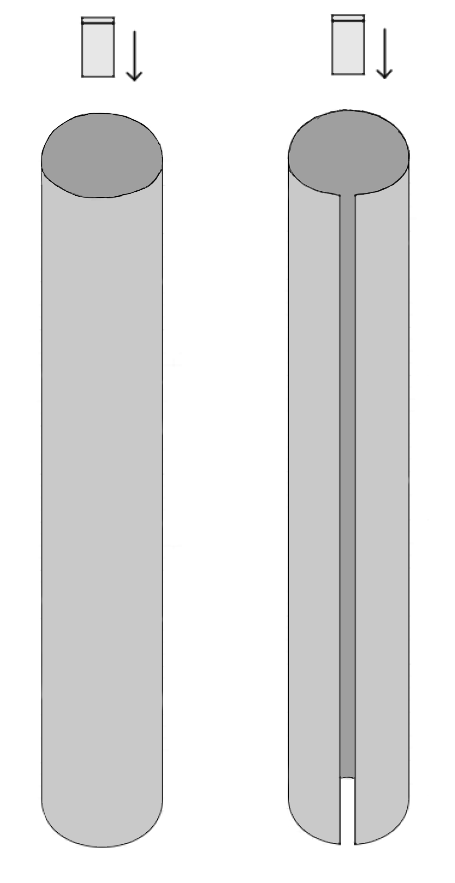
\includegraphics[width=\textwidth]{Neodymmagnet.png}
		\caption{Skizze zum Fallrohr.}
		\label{fig:fallrohr}
	\end{figure}
	
	
\end{document}